%\VignetteIndexEntry{Recovering a Basic Space in R}
%\VignetteKeywords{multivariate}
%\VignettePackage{basicspace}

\documentclass[nojss]{jss}
%\documentclass[article]{jss}
\graphicspath{{Figures/}}

%%%%%%%%%%%%%%%%%%%%%%%%%%%%%%
%% declarations for jss.cls %%%%%%%%%%%%%%%%%%%%%%%%%%%%%%%%%%%%%%%%%%
%%%%%%%%%%%%%%%%%%%%%%%%%%%%%%

%% almost as usual
\author{Keith Poole \\ University of \\ Georgia
  \And
  Jeffrey Lewis \\ University of \\ California, Los Angeles
  \And
  Howard Rosenthal \\ New York\\University
  \And
  James Lo \\ University of \\ Mannheim
  \And
  Royce Carroll \\ Rice University
}
\Plainauthor{Keith Poole, Jeffrey Lewis, Howard Rosenthal, James Lo, Royce Carroll}

\title{Recovering a Basic Space in \proglang{R}}

%% for pretty printing and a nice hypersummary also set:
\Plaintitle{Recovering a Basic Space in R} %% without formatting
%\Shorttitle{A Capitalized Title} %% a short title (if necessary)

%% an abstract and keywords
\Abstract{
\noindent \pkg{basicspace} is a publicly available \proglang{R} package that estimates latent dimensions underlying a set of observable variables, as described in \citet{poole1998recovering}. The scaling procedure effectively performs a singular value decomposition of a rectangular matrix of real elements with missing entries. Monte Carlo tests show that the procedure reliably estimates the latent dimensions and reproduces the missing elements of a matrix even at high levels of error and missing data. In addition, we illustrate applications of the estimator to survey data that is commonly used in the social sciences.
}

\Keywords{multivariate, \proglang{R}, scaling}
\Plainkeywords{multivariate, R, scaling}

%% at least one keyword must be supplied
%% publication information
%% NOTE: Typically, this can be left commented and will be filled out by the technical editor
%% \Volume{13}
%% \Issue{9}
%% \Month{September}
%% \Year{2004}
%% \Submitdate{2004-09-29}
%% \Acceptdate{2004-09-29}

%% The address of (at least) one author should be given
%% in the following format:
\Address{

  Keith T. Poole\\
  Department of Political Science\\
  Baldwin Hall\\
  University of Georgia\\
  Athens, GA 30602\\
  E-mail: \email{kpoole@uga.edu}\\
  URL: \url{http://www.voteview.com/}\\\\

  Jeffrey B. Lewis\\
  University of California - Los Angeles\\
  Political Science Department, Bunche Hall\\
  Los Angeles, CA 90095\\
  E-mail: \email{jblewis@ucla.edu}\\
  URL: \url{http://www.polisci.ucla.edu/faculty/lewis/}\\\\

  Howard Rosenthal\\
  NYU Department of Politics\\
  19 W. 4th Street, New York,  10012\\
  E-mail: \email{howardrosenthal@nyu.edu}\\
  URL: \url{http://politics.as.nyu.edu/object/HowardRosenthal}\\\\

  James Lo\\
  University of Mannheim, SFB 884\\
  L13, 15-17\\
  Mannheim, Germany 68131\\
  E-mail: \email{lo@uni-mannheim.de}\\\\

  Royce Carroll\\
  Department of Political Science, MS 24\\
  Rice University\\
  PO Box 1892\\
  Houston, Texas 77251-1892\\
  E-mail: \email{rcarroll@rice.edu}\\
  URL: \url{http://rcarroll.web.rice.edu/}\\\\

}

%% It is also possible to add a telephone and fax number
%% before the e-mail in the following format:
%% Telephone: +43/1/31336-5053
%% Fax: +43/1/31336-734

%% for those who use Sweave please include the following line (with % symbols):
%% need no \usepackage{Sweave.sty}

%% end of declarations %%%%%%%%%%%%%%%%%%%%%%%%%%%%%%%%%%%%%%%%%%%%%%%


\begin{document}

%% include your article here, just as usual
%% Note that you should use the \pkg{}, \proglang{} and \code{} commands.


\section{Introduction}


This \proglang{R} \citep{R} package contains software designed to recover a latent dimension (i.e. a basic space)
from a numeric matrix of data. The initial development was conducted by \citet{poole1998recovering}, who wrote the Fortran executable that was previously used by social scientists to analyze survey data in publications such as \citet{palfrey1987relationship} and \citet{saiegh2009recovering}.  The principal purpose of the package is to facilitate the analysis of self-placement and/or perceptual survey data by scaling stimuli into a common space.

Stated differently, assume that various political actors (i.e. the stimuli) occupy positions on a continuous left-right political spectrum, and our objective is to recover estimates of those positions.  This package facilitates the estimation of these positions under the assumption that survey respondents report their personal estimates of these positions with different levels of bias and scale attenuation. While intended for use with survey data, this procedure has potentially broader applications outside of social science because mathematically it is a special case of singular value decomposition on a numeric matrix with missing data.\footnote{When used to analyze survey data, this property implies that survey scales can be treated as a continuous rather than ordinal variable. Researchers who believe that their scales are ordinal should therefore not be using the model presented here.}

This paper proceeds in four steps. First, we begin with a description of the mathematics that underlie the basic space estimator. We then provide three examples. First, we show a Monte Carlo analysis that suggests our estimator produces an accurate decomposition of our simulated data matrices even with 30 per cent of the data missing. Stated differently, we are able to estimate an Eckart-Young lower-rank approximation matrix of a matrix with missing entries.   Secondly, we show how the procedure can be applied to self-placement survey data from the  1980 National Election Survey. Next, we proceed with an application of the model to perceptual data from the 1980 National Election Study, where various political candidates are ranked along a 7 point liberal-conservative scale. We conclude with a look at a related estimator developed by \citet{aldrich1977method} that is also included in this package for historical purposes.


\section{Model}

The exposition of the model presented here closely follows \citet{poole1998recovering}. Consider a matrix of survey data $X_0$ with $n$ respondents and $m$ issue scales, with individuals on the rows and issues on the columns. Some cells of the matrix $X_0$ are missing, and we let $X$ denote the version of $X_0$ that has no missing data. In each cell $x_{ij}$, respondent $i$ (\textit{i=1, \ldots, n}) reports their position on issue scale $j$ (\textit{j=1, \ldots, m}), with some responses missing.\footnote{The `0' subscript indicates that some elements are missing from the matrix.} Now let $\Psi_{ik}$ be the $i$th individual's position on the $k$th basic dimension (\textit{k=1, \ldots, s}), $W$ be an $m$ by $s$ matrix of weights that map individual positions from the basic space to the issue dimensions, $c$ be a vector of issue dimension intercept terms of length $m$, $J_n$ by an $n$ length vector of ones, and $E_0$ be error terms in the data matrix. The model that we seek to estimate is:

\begin{equation}
X_0 = [\Psi W' + J_nc']_0 + E_0
\label{one}
\end{equation}

Without loss of generality, we also assume that $E_0$ is drawn from a symmetric distribution with
mean 0 and the centroid of the basic space coordinates is at the origin (i.e. $J_n'\Psi=0$).
Substituting into the model equation, this implies that $J_n'[X-J_nc'] = 0_m'$, where $0_m$ is an $m$
length vector of zeroes. Then in the situation where $X_0$ has no missing data, the parameters
of interest can all be recovered using singular value decomposition.  To see why this is true, recall
that for an $n$ by $m$ matrix of real elements with $n \ge m$, there exists an $n$ by $m$ orthogonal
matrix $U$, an $m$ by $m$ orthogonal matrix $V$, and an $m$ by $m$ matrix $\Lambda$ such that:

\begin{equation}
X = U \Lambda V'
\label{two}
\end{equation}

\noindent where $\Lambda$ is a diagonal matrix of singular values.\footnote{A more general
form of this equation can be written in which $\Lambda$ is instead an $n$ by $m$ matrix and $U$ is
$n$ by $n$.} To solve (\ref{one}), set $c$ equal to the column means of $X$, or $c_j = \frac{\sum\limits_{i=1}^n x_{ij}}{n} = \bar{x}_j$. Then using (\ref{two}), the singular value decomposition of $X - J_nc'$ can be expressed as:

$$X - J_nc'\ =\ U \Lambda V'\ =\ \Psi W'$$

This implies that in the absence of missing data, one solution for $\Psi$ and $W$ is:

$$\Psi = U\Lambda^{0.5}$$

$$W = V\Lambda^{0.5}$$

\noindent with $\Lambda^{0.5}$ being a diagonal matrix where diagonal elements are the square roots of $\Lambda$. While other solutions to this problem exist, \citet{eckart1936approximation} have shown that the least squares approximation in $s$ dimensions of a matrix $A$ can be found by using only the first $s$ singular values of $A$ along the diagonal of $\Lambda$ and re-multiplying $U \Lambda V'$.

In the presence of missing data in data matrix $X_0$, the use of singular value decomposition
to solve for $W$ and $\Psi$ is no longer possible, and we instead estimate $\hat{W}$ and
$\hat{\Psi}$ using an alternating least squares (ALS) technique that is similar to the procedures
used in \citet{carroll1970analysis} and \citet{takane1977nonmetric}. The objective
function to be minimized is the sum of the squared deviations across all cells in $A$ after
the columns have been adjusted for column means, or:

$$\xi = \displaystyle\sum\limits_{i=1}^n \sum\limits_{j=1}^{m_i} \{[ \sum\limits_{k=1}^s \Psi_{ik}W_{jk}] + c_j -x_{ij} \}^2$$

In minimizing this objective function, two constraints from the earlier analysis with no missing
data are applied. First, we exploit the the fact that $\Psi$ and $W$ are orthogonal matrices, which implies
that $\Psi'\Psi = W'W$.\footnote{More specifically, $\Psi'\Psi = \Lambda^{0.5}U'U\Lambda^{0.5} = \Lambda^{0.5}I_m\Lambda^{0.5} = \Lambda = W'W.$} Secondly, following our earlier restriction that $J_n'[X-J_nc'] = 0_m'$, $J_n'U = J_n'\Psi = 0_m'$ as well.
These restrictions produce the Lagrangian multiplier problem:


$$\mu = \xi = 2\gamma'['\Psi'J_n] + tr[\Phi(\Psi'\Psi - W'W)]$$

\noindent where $\Phi$ is a symmetric $s$ by $s$ matrix of Lagrangian multipliers and $\gamma$ is an $s$ length
vector of Lagrangian multipliers. Since all Lagrangian multipliers are zero,\footnote{See Appendix A in \citet{poole1998recovering}
for a full proof that all Lagrangian multipliers are zero.} the partial derivatives of $\xi$ are:

\begin{equation}
\frac{\partial \mu}{\partial \Psi_{ik}} = 2\displaystyle\sum\limits_{j=1}^{m_i} [(\sum\limits_{l=1}^s w_{jl}\psi_{jl})+ c_j - x_{ij}]w_{jk}
\label{three}
\end{equation}

\begin{equation}
\frac{\partial \mu}{\partial w_{jk}} = 2\displaystyle\sum\limits_{i=1}^{n_j} [(\sum\limits_{l=1}^s w_{jl}\psi_{jl})+ c_j - x_{ij}]\psi_{jk}
\label{four}
\end{equation}

\begin{equation}
\frac{\partial \mu}{\partial c_j} = 2\displaystyle\sum\limits_{i=1}^{n_j} [(\sum\limits_{l=1}^s w_{jl}\psi_{jl})+ c_j - x_{ij}]
\label{five}
\end{equation}

Let $W^*$ be an $m_i$ by $s$ matrix with appropriate rows corresponding to missing entries in $X_0$ removed, $x_{0i}$ be the
length $m_i$ row of $X_0$, and $c_0$ be the length $m_i$ vector of constants corresponding to the elements of $x_{0i}$. Then
if $W^*$'$W^*$ exists, the $ith$ row of $\Psi$ can be estimated by setting (\ref{three}) to zero, collecting the $s$ partial derivatives
of the $i$th row of $\Psi$ into a vector and solving for $\psi_j$ as:

\begin{equation}
\hat{\psi}_i = (W^*\mathrm{'}W^*)^{-1} W^*\mathrm{'}[x_{0i} - c_{0}]
\label{six}
\end{equation}

\noindent which can of course by estimated using ordinary least squares. Similarly, let $\Psi_j^* = [\Psi_0|J_0]$ be an
$n_j$ by $s+1$ matrix with the appropriate rows corresponding to missing data removed and bordered by ones, $w_j$ be
the $s$ length vector of row $j$ in $W$, $c_j$ be the $j$th element of $c$, and $x_{0j}$ be the $j$th column of $X_0$.
Then if $\Psi_{j}^*$$'\Psi_j^*$ exists, $w_j$ and $c_j$ can be jointly estimated by combining (\ref{four}) and (\ref{five}) as:

\begin{equation}
\frac{\hat{w}_j}{\hat{c}_j} = (\Psi_j^*\mathrm{'}\Psi_j^*)^{-1} \Psi_j^*\mathrm{'}x_{0j}
\label{seven}
\end{equation}

Equations (\ref{six}) and (\ref{seven}) represent the core set of equations that are used to solve for $\hat{W}$,
$\hat{c}$, and $\hat{\Psi}$. Once a set of starting values has been generated, (\ref{six}) and (\ref{seven}) are
iterated until convergence is complete. Generation of appropriate start values is conducted one dimension at a time,
and a more detailed justification of the procedure can be found in \citet{poole1998recovering}. On the first dimension, start
values are generated by using the following three equations:

\begin{equation}
\hat{c}_{j} = \frac{\displaystyle\sum\limits_{j=1}^{n_j} x_{ij}}{n_j} = \bar{x}_j
\label{eight}
\end{equation}

\begin{equation}
w_{j1} = diag(\Gamma)
\label{nine}
\end{equation}

\noindent where $\Gamma$ is an $m$ by $m$ diagonal matrix with diagonal elements either set to 1 or -1
that maximizes the number of positive elements in the $m$ by $m$ covariance matrix
$\Gamma[X_0 - J_nc']\mathrm{'}[X_0 - J_nc']\Gamma$. $\Gamma$ is found by a simple iterative process
similar to that used to speed eigenvector/eigenvalue decomposition \citep{poole1998recovering}. Given equations (\ref{eight})
and (\ref{nine}), starting values for $\psi$ are:

\begin{equation}
\hat{\psi}_{i1} = \frac{\displaystyle\sum\limits_{j=1}^{m_i} \hat{w}_{j1}(x_{ij}-\hat{c}_j)}{m_i}
\label{ten}
\end{equation}

If more than one dimensions are to be estimated ($s > 1$), start values for other dimensions can be generated
simply by replacing the data matrix $X_0$ with the matrix of residuals $E_{0s}$ in equations (\ref{nine}) and (\ref{ten}). However, no further estimation of start values for $\hat{c}$ is required. The matrix of residuals to be used for generating start values on dimension $s$ is:

$$E_{0s} = X_0 - \displaystyle\sum\limits_{j=1}^{s} \hat{\Psi}_s\hat{w}_s\mathrm{'} - J_n\hat{c}'$$

This residual matrix allows the generation of higher-dimension start values by iterating $\Gamma$ to
maximize the positive elements in $E_{0s}$. The starting values are now:

%Equation 12 in paper
\begin{equation}
\hat{\psi}_{is} = \frac{\displaystyle\sum\limits_{j=1}^{m_i} \hat{w}_{js}e_{1(s-1)ij}}{\sum\limits_{j=1}^{m_j} \hat{w}_{js}^2}
\label{eleven}
\end{equation}

\noindent where the initial $\hat{w_{js}}$ values of +1s and -1s are used to obtain $\hat{\psi}_{is}$ starting values. The starting values of $\hat{w_{js}}$ are now:

%Equation 11 in paper
\begin{equation}
\hat{w}_{js} = \frac{\displaystyle\sum\limits_{i=1}^{n_j} \hat{\psi}_{is}e_{(s-1)ij}}{\sum\limits_{i=1}^{n_j} \hat{\psi}_{is}^2}
\label{twelve}
\end{equation}


Summarizing the preceding discussion in full, the basic space technique decomposes an $n$ by $m$ matrix $X_0$ with
$n > m$ following equation (\ref{one}). In the absence of missing data, this decomposition can be solved using
singular value decomposition as in equation (\ref{two}). The basic space technique can therefore be thought of as
a generalization of singular value decomposition to matrices with missing data. Estimation of (\ref{one}) proceeds
in three steps. In the first stage, starting values on the first dimension are generated for $\hat{c}_{j}$, $w_{j1}$,
and $\hat{\psi}_{i1}$ by iterating equations (\ref{eight})-(\ref{ten}) until convergence. In the second stage, if the
number of dimensions to be estimated $s > 1$, higher dimensional starting values for $\hat{\psi}_{is}$ and $\hat{w}_{is}$
are generated dimension by dimension using equations (\ref{eleven})-(\ref{twelve}). Finally, the starting values generated 
in the preceding two stages are improved by iterating equations (\ref{six})-(\ref{seven}) until convergence.

\section{Monte Carlo Test}

In this section, we present the first of four motivating examples. We begin with a Monte Carlo example that
tests the basic space technique against simulated data. Four key variables should be set in each simulation:
the number of respondents $N$ (set here to $N=1000$), the number of issue scales (also referred to as stimuli,
and set here to $M=20$), the number of explanatory dimensions (set here to $s=2$), the
fraction of observations that are missing (set here as 0.3), and the distribution of error terms (set here as
random uniform draws from -0.5 to 0.5). These variables can be changed for other simulations, but the
restriction that $N>M$ must be hold true. In cases where $M>N$ please refer to the third example that uses
\code{blackbox\_transpose} and \code{aldmck}.

\begin{Schunk}
\begin{Sinput}
> set.seed(1231)
> library(basicspace)
\end{Sinput}
\begin{Soutput}
## BASIC SPACE SCALING PACKAGE 
## Copyright 2009 - 2011 
## Keith Poole, Howard Rosenthal, Jeffrey Lewis, James Lo, and Royce Carroll
## Support provided by the U.S. National Science Foundation
## NSF Grant SES-0611974
\end{Soutput}
\begin{Sinput}
> N <- 1000
> M <- 20
> s <- 2
> fraction.missing <- 0.3
> E <- matrix(runif(N * M, min = -0.5, max = 0.5), 
+     nrow = N, ncol = M)
\end{Sinput}
\end{Schunk}

To generate the $X$ matrix (i.e. the matrix in (\ref{one}) before missing values are introduced), separately
generate the matrices that produce the singular value decomposition of $X$ following (\ref{two}). Also
generate the $J_n$ and $c$ vectors from (1). While $X$ can be generated directly in one step, creating the
components separately enjoys two significant advantages. First, recovery of the true values of $\Psi$ and $W$
is simplified. Secondly, the creation of $\Lambda$ separately allows us to more easily tune the dimensionality
of the matrix as desired.

\begin{Schunk}
\begin{Sinput}
> U <- matrix(runif(N * s), nrow = N, ncol = s)
> D <- diag(seq(from = 2.1, by = -0.2, length.out = s))
> V.prime <- matrix(runif(s * M), nrow = s, ncol = M)
> c <- rnorm(M)
> Jn <- rep(1, N)
\end{Sinput}
\end{Schunk}

With the intermediate matrices just generated, we can produce our $X$ matrix by using equation (\ref{one})
and the true $\Psi$ and $W$ matrices using: $\Psi = U\Lambda^{0.5}$ and $W = V\Lambda^{0.5}$. 

\begin{Schunk}
\begin{Sinput}
> X.true <- U %*% D %*% V.prime + Jn %o% c
> X.0 <- X.true + E
> Psi.true <- U %*% sqrt(D)
> W.true <- t(V.prime) %*% sqrt(D)
\end{Sinput}
\end{Schunk}

$X_0$ is simply the $X$ matrix with missing data values included completely at random, so we insert
our missing data code (999 in the example) into the appropriate fraction of values as follows:

\begin{Schunk}
\begin{Sinput}
> missing <- sample(1:(N * M), round(fraction.missing * 
+     N * M))
> X.0[missing] <- 999
\end{Sinput}
\end{Schunk}

The final step before estimation is to assign row and column names to the data set prior to input. In
most applications these names are generally pulled from a survey, but they can also be generated
manually:

\begin{Schunk}
\begin{Sinput}
> rownames(X.0) <- paste("Legis", 1:N, sep = "")
> colnames(X.0) <- paste("V", 1:M, sep = "")
\end{Sinput}
\end{Schunk}

Estimation of the Monte Carlo data after formatting is trivial. The function that applies the basic space
decomposition described in this paper is \code{blackbox}.  It takes four arguments: the matrix to
be decomposed, a vector of missing data values, a boolean flag indicating whether verbose output is
desired, the number of dimensions to estimate, and the minimum number of issue scales that an individual
needs to provide responses to if they are to be included in the estimation.

\begin{Schunk}
\begin{Sinput}
> result <- blackbox(X.0, missing = c(999), verbose = TRUE, 
+     dims = 2, minscale = 8)
\end{Sinput}
\begin{Soutput}
	Beginning Blackbox Scaling...20 stimuli have been provided.

	Blackbox estimation completed successfully.
\end{Soutput}
\begin{Sinput}
> names(result)
\end{Sinput}
\begin{Soutput}
[1] "stimuli"     "individuals" "fits"        "Nrow"       
[5] "Ncol"        "Ndata"       "Nmiss"       "SS_mean"    
[9] "dims"       
\end{Soutput}
\end{Schunk}

The output object contains multiple data frames summarizing the results of the estimation. The key data
frames are \code{stimuli}, which contain estimates of $\hat{W}$ and $\hat{c}$, as well as \code{individuals},
which contain estimates of $\hat{\Psi}$.  The other quantities are fit statistics described in greater
detail in the standard documentation for the function.

With the estimates complete, we are now able to test the recovery of our parameters of interest. In general,
scaling problems are not fully identified. Stated differently, given $X = \Psi W'$, $\Psi$ and $W'$ are not
unique solutions because $X = \Psi K K^{-1} W'$ for any conformable and invertible matrix $K$, so $X$ can
always be decomposed instead as $X = \Psi^* W^{*'}$ where $\Psi^* = \Psi K$ and $W^{*'} = K^{-1} W'$. 
When evaluating parameter fit, we are therefore largely concerned with finding monotonic relationships between
the true and estimated parameters of interest.  Figure \ref{fig:seven} compares the true vs. estimated values of
$\Psi$ across two dimensions, and the results suggest a reasonable model fit.

\begin{figure}
\begin{center}
\begin{Schunk}
\begin{Sinput}
> par(mfrow = c(1, 2))
> plot(Psi.true[, 1], result$individuals[[2]]$c1, 
+     xlim = c(0, 1.5), ylim = c(-0.65, 0.6), pch = 20, 
+     cex = 0.4, cex.lab = 1.6, bty = "n", xlab = "True Psi, first dimension", 
+     ylab = "Recovered Psi, first dimension")
> plot(Psi.true[, 2], result$individuals[[2]]$c2, 
+     xlim = c(0, 1.5), ylim = c(-0.65, 0.6), pch = 20, 
+     cex = 0.4, cex.lab = 1.6, bty = "n", xlab = "True Psi, second dimension", 
+     ylab = "Recovered Psi, second dimension")
\end{Sinput}
\end{Schunk}
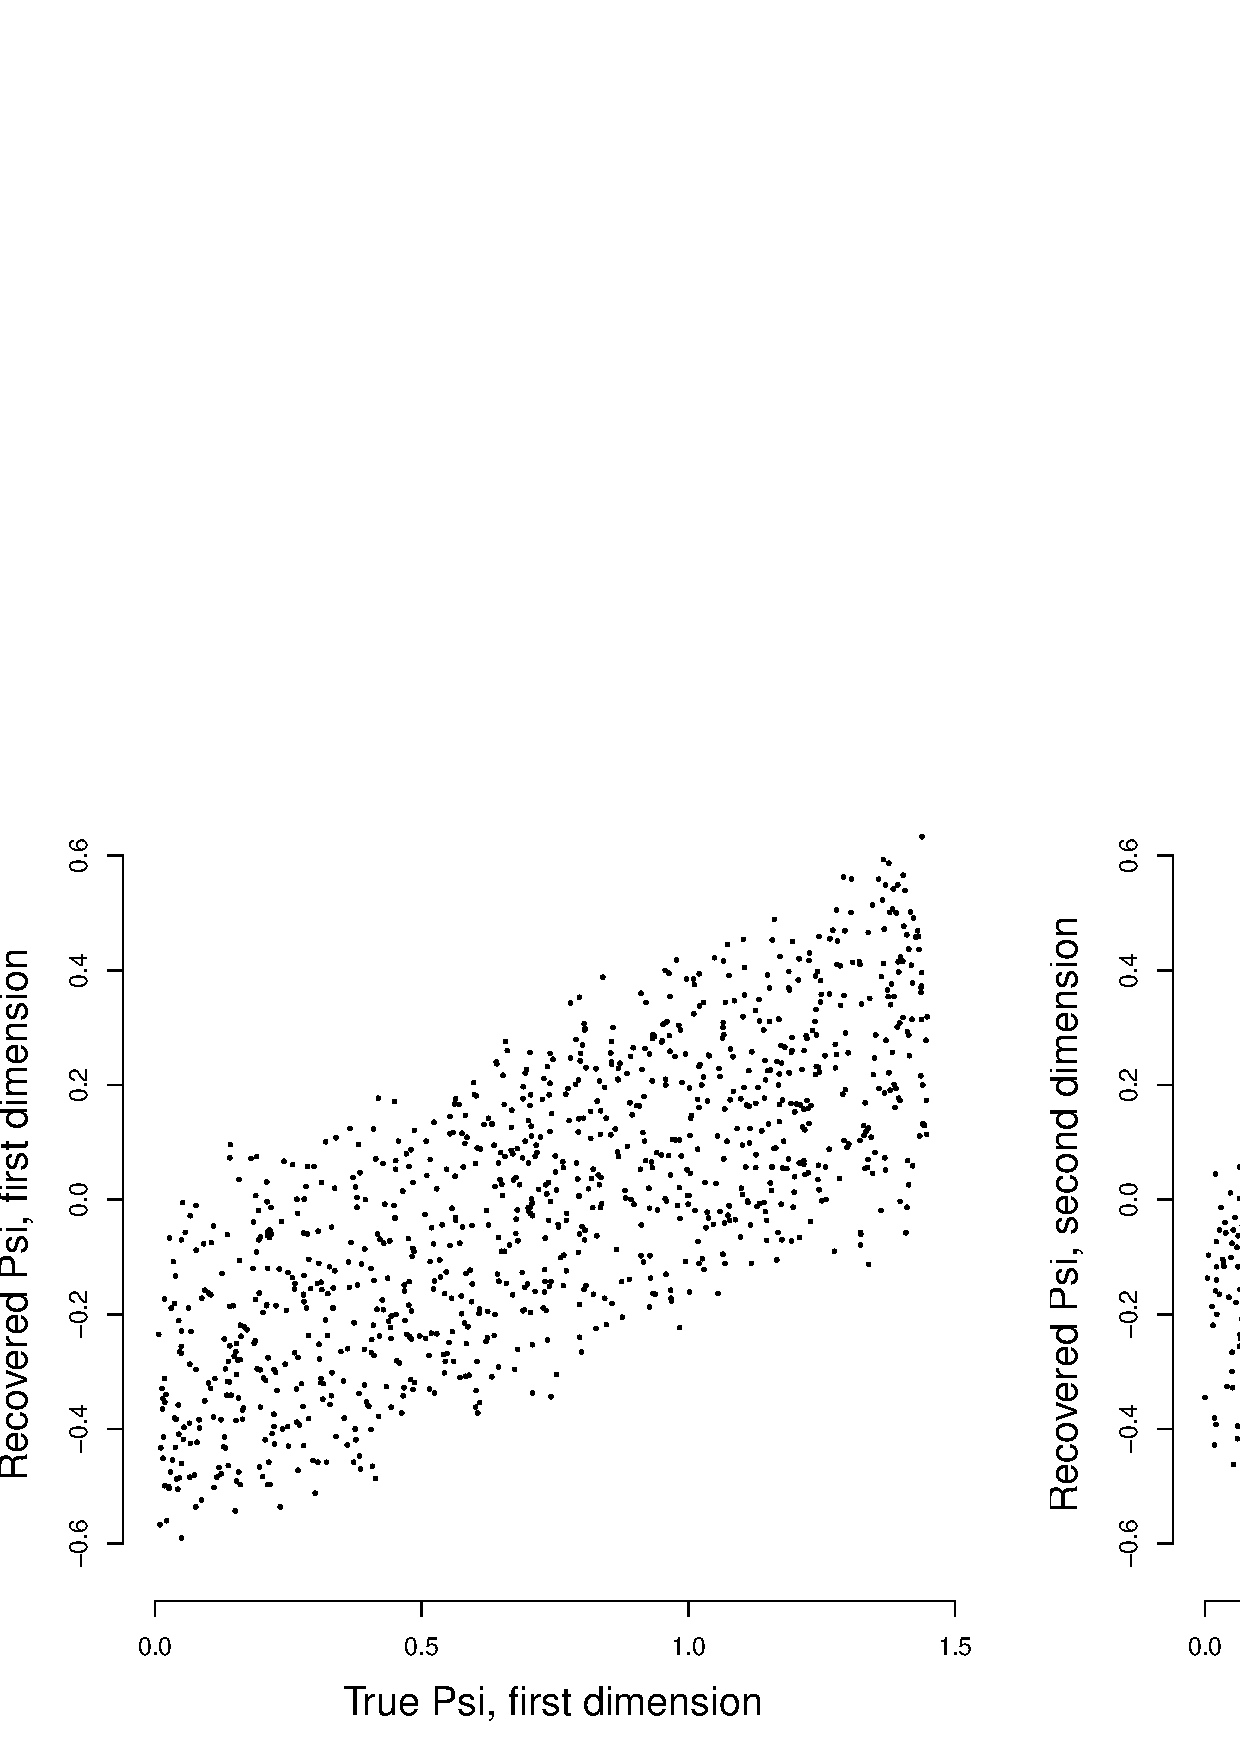
\includegraphics{basicspace-seven}
\end{center}
\caption{Plots of True vs. Estimated $\Psi$ scores, first and second dimension.}
\label{fig:seven}
\end{figure}

Figure \ref{fig:six} shows the results for the same procedure applied to $W$. In Figure
\ref{fig:eight} we repeat this analysis for $c$, which is a column mean that is only estimated in
one dimension.  In both cases the estimates for $\hat{W}$ and $\hat{c}$ are a monotonic transformation of the
true parameters as expected.\footnote{In other estimates, the relationship may only be affine because $X = \Psi W'$
implies $X = -(\Psi) -(W')$ as well.}

\begin{figure}
\begin{center}
\begin{Schunk}
\begin{Sinput}
> par(mfrow = c(1, 2))
> plot(W.true[, 1], result$stimuli[[2]]$w1, ylim = c(1, 
+     2.6), pch = 20, cex = 1.5, cex.lab = 1.6, 
+     bty = "n", xlab = "True W, first dimension", 
+     ylab = "Recovered W, first dimension")
> plot(W.true[, 2], result$stimuli[[2]]$w2, ylim = c(-2, 
+     2), pch = 20, cex = 1.5, cex.lab = 1.6, bty = "n", 
+     xlab = "True W, second dimension", ylab = "Recovered W, second dimension")
\end{Sinput}
\end{Schunk}
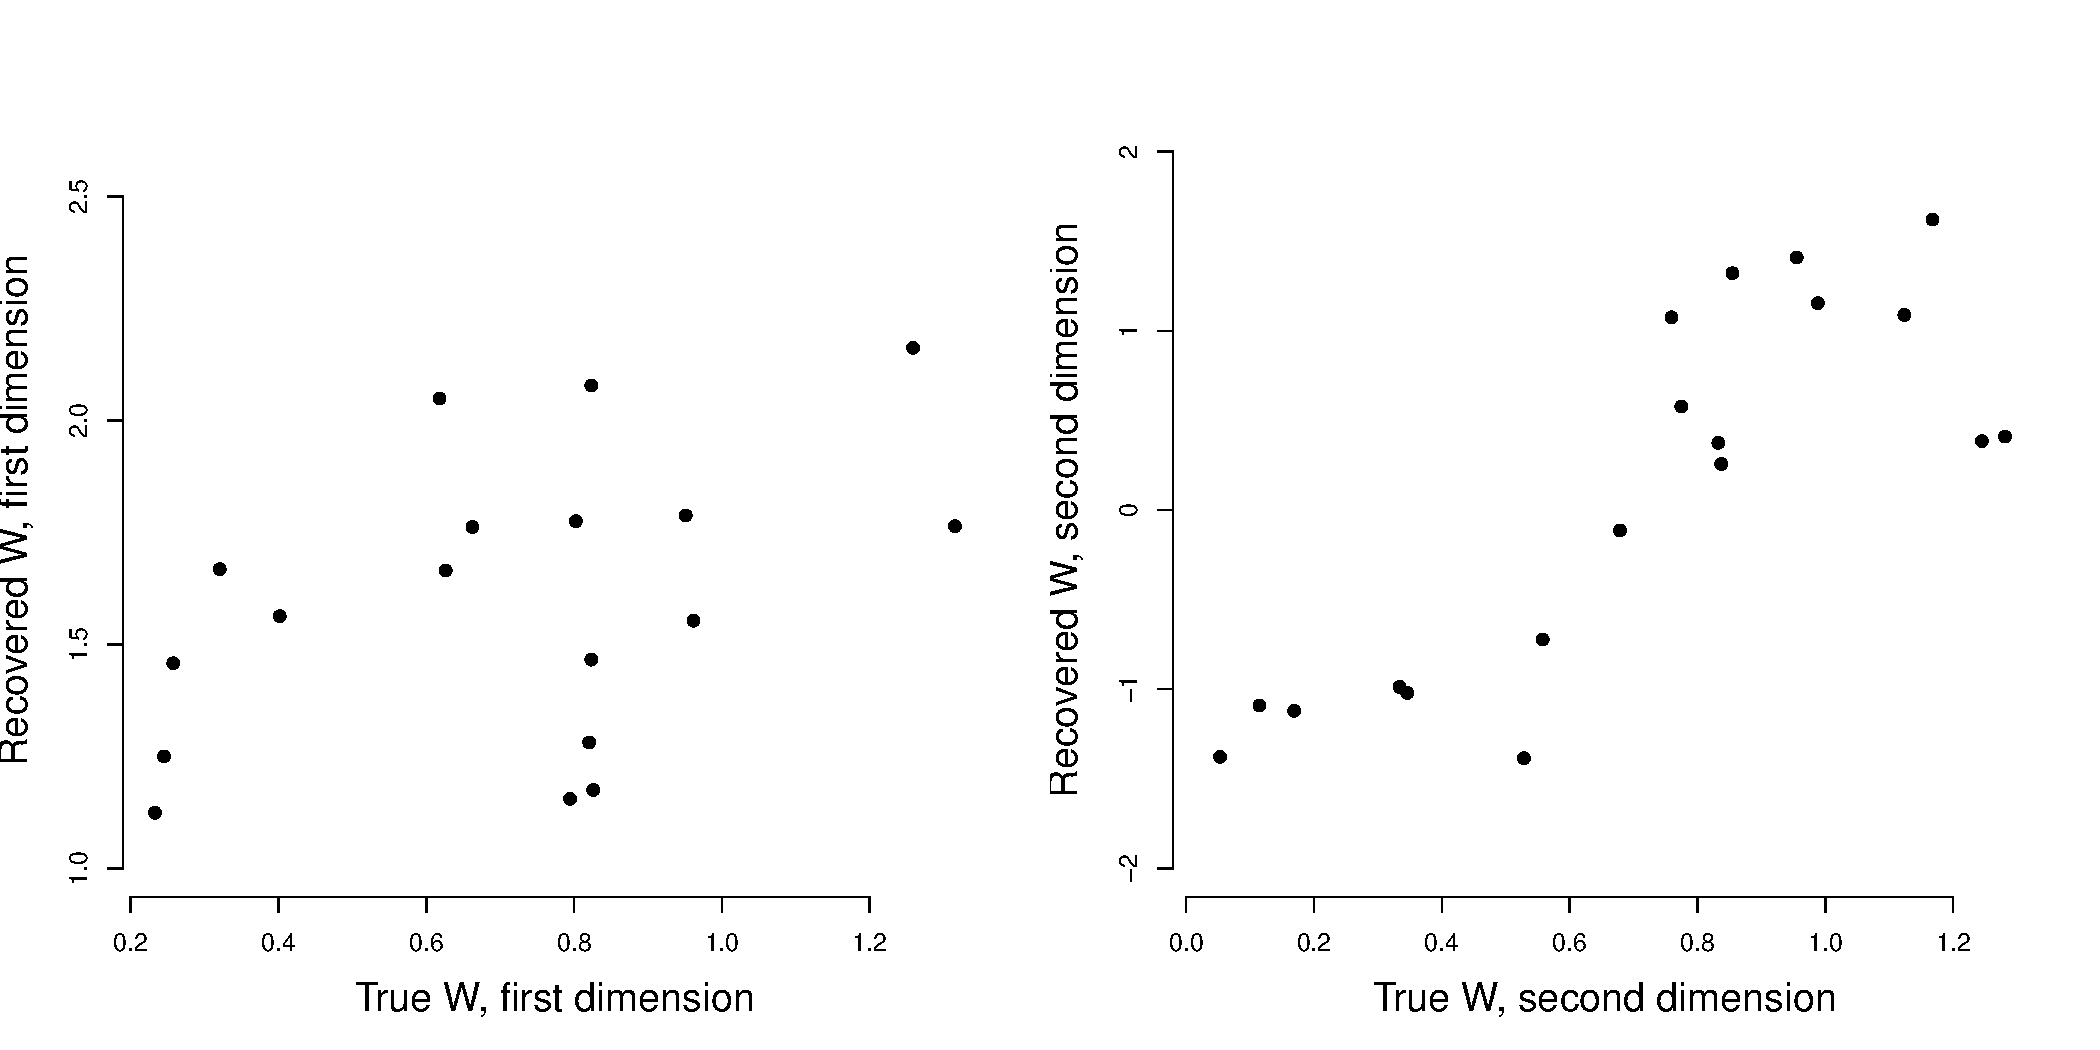
\includegraphics{basicspace-six}
\end{center}
\caption{Plots of True vs. Estimated $W$ scores, first and second dimension.}
\label{fig:six}
\end{figure}


\begin{figure}
\begin{center}
\begin{Schunk}
\begin{Sinput}
> par(mfrow = c(1, 1))
> plot(c, result$stimuli[[2]]$c, pch = 20, cex = 1.2, 
+     cex.lab = 1.1, bty = "n", xlab = "True C", 
+     ylab = "Recovered C")
\end{Sinput}
\end{Schunk}
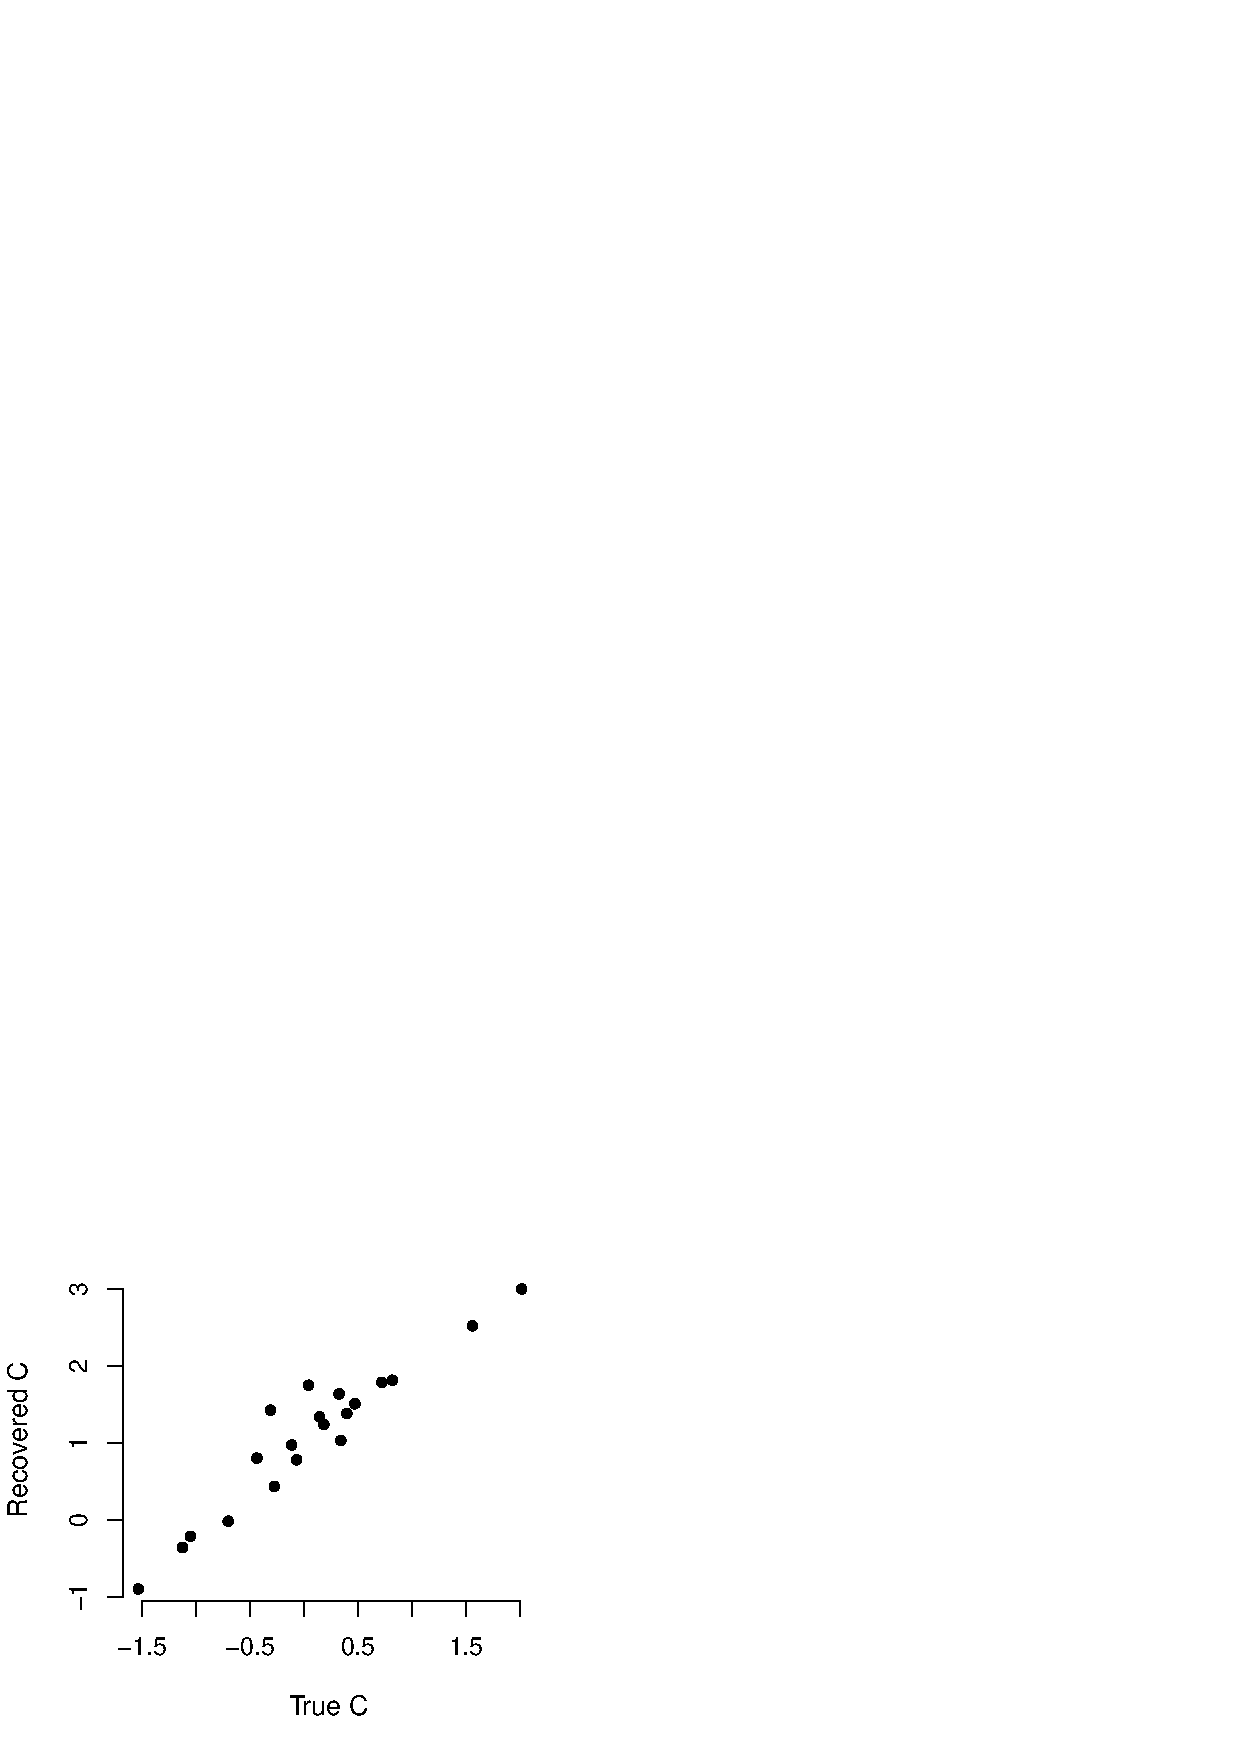
\includegraphics{basicspace-eight}
\end{center}
\caption{Plot of True vs. Estimated $c$ scores.}
\label{fig:eight}
\end{figure}

Finally, we pool our estimates of $\hat{W}$, $\hat{\Psi}$, and $\hat{c}$ together to
estimate the full matrix $\hat{X}$ following Equation ($\ref{one}$).  While social
scientists are principally concerned with estimation of $\hat{W}$ and $\hat{\Psi}$,
others seeking to conduct singular value decomposition of matrices with missing
data may find $\hat{X}$ to be of value. One obvious application of $\hat{X}$ is
its potential use as an imputation tool for missing data.\footnote{The simulation
presented here simulates missing data under the Missing Completely at Random (MCAR)
assumption --- nevertheless, there is no reason to think that this would not work
under conditions where data are instead Missing at Random (MAR).} To test the viability
of this idea, we separately plot the true values of $X$ against the estimated values
of $\hat{X}$ separately for the cells retained in the estimation, and compared
those results to estimates of $\hat{X}$ in cells that were discarded prior to estimation
to simulate the missing data mechanism. Figure \ref{fig:nine} presents our results for retained vs.
imputed X. What is particularly notable about this result is the close similarity
between these plots --- the imputed values not only appear reasonable (i.e. line up
with the true values along a $45^{\circ}$ line), but imputed values do not appear to have
significantly higher mean squared error than the values that were retained (i.e. variance
along the $45^{\circ}$ line is similar in both plots). While further tests are necessary,
these results suggest that the use of the techniques demonstrated here may have greater
applicability beyond survey research.  Further discussion of imputation can be found in the
unpublished appendix to \citet{poole1998recovering}.


\begin{figure}
\begin{center}
\begin{Schunk}
\begin{Sinput}
> W.hat <- cbind(result$stimuli[[2]]$w1, result$stimuli[[2]]$w2)
> Psi.hat <- cbind(result$individuals[[2]]$c1, result$individuals[[2]]$c2)
> X.hat <- Psi.hat %*% t(W.hat) + Jn %o% result$stimuli[[2]]$c
> par(mfrow = c(1, 2))
> plot(X.true[missing], X.hat[missing], pch = 20, 
+     cex = 0.4, cex.lab = 1.2, bty = "n", xlab = "True X, missing values", 
+     ylab = "Recovered X, missing values")
> plot(X.true[!(1:(N * M) %in% missing)], X.hat[!(1:(N * 
+     M) %in% missing)], pch = 20, cex = 0.4, cex.lab = 1.2, 
+     bty = "n", xlab = "True X, nonmissing values", 
+     ylab = "Recovered X, nonmissing values")
\end{Sinput}
\end{Schunk}
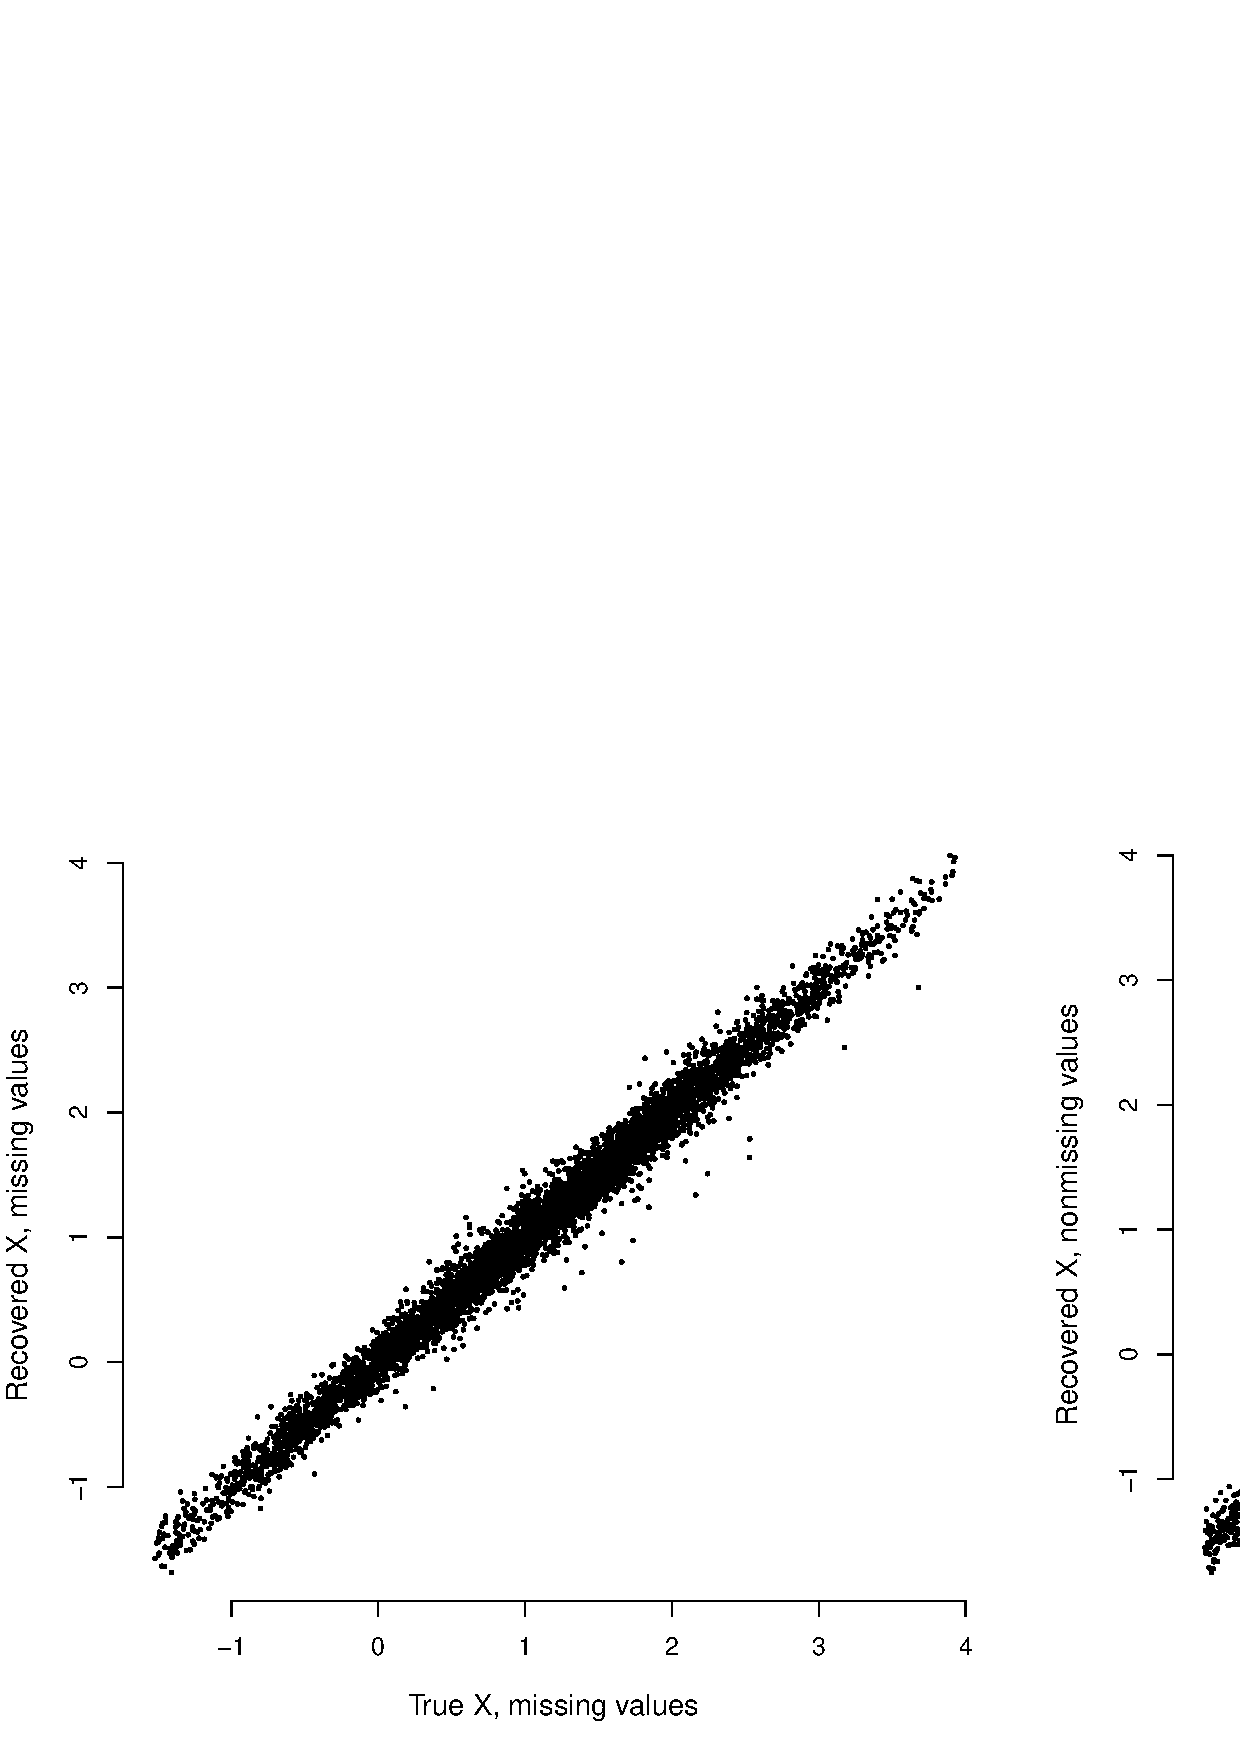
\includegraphics{basicspace-nine}
\end{center}
\caption{Plots of True vs. Estimated $X$ scores for missing vs. nonmissing values.}
\label{fig:nine}
\end{figure}


\section{Example 1: 1980 NES Issue Scales}

In this section we present an application of the basic space model to a common problem in social science.
One issue of interest to political scientists in particular are empirical models of voting (also
known as ideal point models), that allow legislator locations in an abstract policy or ideological space
to be inferred from their roll call votes. The recovered scores have wide applicability to the study
of Congress \citep{Congress, app1}, elections \citep{herronlewis},
courts \citep{martin2002dynamic}, and in non-legislative voting bodies such as the United
Nations \citep{Voeten}.\footnote{For a more extensive review of applications of spatial modeling
in the social sciences, see \citet{poole2005spatial}.}  The most prominent ideal point model in the political
science literature is NOMINATE \citep{Congress}, a model that estimates the policy
preferences of legislators using observed roll call votes as the primary source of data.\footnote{The
\pkg{wnominate} package on CRAN contains software used to estimate NOMINATE scores.}  However, the
use of models such as NOMINATE may not always be possible because roll call data is often not
available or recorded.  In such instances, the basic space model shown here presents an attractive
alternative estimator.\footnote{For a more comprehensive review of the advantages and disadvantages
of different data sources for spatial models, see \citet{saiegh2009recovering}.}

We present a simple example that applies the basic space model to a set of issue scales from the
1980 National Election Study. This survey contains N=1,614 respondents who were asked to place themselves
on scales about desired levels of defense spending, inflation, tax cuts, abortion, liberal-conservative
scales, the role of women, the role of government in providing jobs, busing, and other similar issues.
We assume that each respondent has a location in a common ideological space and attempt to recover
estimates of those locations, which is represented as $\Psi$ in (\ref{one}). In providing responses
to the issue scales, each respondent reports their true ideological position $\Psi$, modified by a
stretch parameter $W$ and an additive intercept parameter $c$ along with noise $E_0$. The data is simply
stored in a standard matrix or data frame with respondents on the rows and survey questions (i.e. stimuli)
on the columns as follows:

\begin{Schunk}
\begin{Sinput}
> data(Issues1980)
> Issues1980[1:10, 1:4]
\end{Sinput}
\begin{Soutput}
   libcon1 defense govserv inflation
1        0       7       5         4
2        4       4       6         7
3        6       3       0         0
4        5       6       2         8
5        3       4       2         4
6        5       5       4         0
7        8       2       6         5
8        2       7       7         6
9        6       7       2         2
10       5       4       2         5
\end{Soutput}
\end{Schunk}

Virtually all surveys contain missing data, and for the two survey questions about abortion, `7' is
used as a missing data code. However, many of the other scales in this data set us 7 point scales, so
we need to recode the missing data for those questions.

\begin{Schunk}
\begin{Sinput}
> Issues1980[Issues1980[, "abortion1"] == 7, "abortion1"] <- 8
> Issues1980[Issues1980[, "abortion2"] == 7, "abortion2"] <- 8
\end{Sinput}
\end{Schunk}

Estimation of the scores is now trivial using the \code{blackbox} function, which takes the same
arguments already described in the Monte Carlo example:

\begin{Schunk}
\begin{Sinput}
> result <- blackbox(Issues1980, missing = c(0, 
+     8, 9), verbose = FALSE, dims = 3, minscale = 8)
\end{Sinput}
\end{Schunk}

Objects of class \code{blackbox} can also be summarized using the \code{summary} function, although
the summaries largely provide only summaries of the stimuli. For each dimension estimated, the summary
provides the intercept ($c$) and stretch ($w_1 \ldots w_3$) parameters for each question, as well
as the number of respondents and various fit statistics.

\begin{Schunk}
\begin{Sinput}
> summary(result)
\end{Sinput}
\begin{Soutput}
SUMMARY OF BLACKBOX OBJECT
----------------------------------
               N     c     w1    R2
libcon1      875 4.280 -3.028 0.414
defense     1163 5.210 -1.754 0.123
govserv     1119 4.323  4.302 0.450
inflation    816 4.106  2.015 0.159
abortion1   1238 2.856  0.627 0.031
taxcut       836 2.839 -1.074 0.055
libcon2      949 4.369 -2.755 0.414
govhelpmin  1160 4.542 -3.400 0.412
russia      1152 3.891 -3.034 0.231
womenrole   1223 2.845 -2.866 0.204
govjobs     1131 4.377 -4.488 0.518
equalrights 1144 2.663 -3.297 0.381
busing      1219 6.051 -2.699 0.255
abortion2   1246 2.675  0.724 0.047

               N     c     w1     w2    R2
libcon1      875 4.300 -2.966  0.954 0.424
defense     1163 5.214 -1.779  0.899 0.147
govserv     1119 4.368  4.331  3.042 0.617
inflation    816 4.152  2.088  2.940 0.393
abortion1   1238 2.856  0.512 -2.211 0.290
taxcut       836 2.818 -1.103 -0.667 0.071
libcon2      949 4.377 -2.758  0.459 0.423
govhelpmin  1160 4.535 -3.456 -0.119 0.424
russia      1152 3.887 -3.140  0.241 0.247
womenrole   1223 2.872 -2.466  6.007 0.771
govjobs     1131 4.350 -4.595 -2.417 0.635
equalrights 1144 2.673 -3.148  2.438 0.491
busing      1219 6.049 -2.741  0.059 0.263
abortion2   1246 2.676  0.629 -2.112 0.318

               N     c     w1     w2     w3    R2
libcon1      875 4.294 -2.976  0.708 -1.180 0.448
defense     1163 5.200 -1.806  1.586  2.562 0.315
govserv     1119 4.410  4.295  3.707  2.929 0.778
inflation    816 4.169  1.998  3.286  1.111 0.451
abortion1   1238 2.856  0.497 -2.004  1.174 0.312
taxcut       836 2.813 -1.049 -0.902 -0.891 0.091
libcon2      949 4.367 -2.785  0.265 -0.557 0.437
govhelpmin  1160 4.534 -3.457  0.140  0.961 0.440
russia      1152 3.831 -3.255  1.558  5.590 0.695
womenrole   1223 2.891 -2.372  5.602 -2.868 0.805
govjobs     1131 4.341 -4.632 -2.176  1.392 0.648
equalrights 1144 2.680 -3.159  1.860 -2.372 0.563
busing      1219 6.042 -2.819  0.329  1.282 0.306
abortion2   1246 2.675  0.587 -1.980  0.906 0.329

	Dimensions Estimated: 3
	Number of Rows: 1270
	Number of Columns: 14
	Total Number of Data Entries: 15271
	Number of Missing Entries: 2509
	Percent Missing Data: 14.11%
	Sum of Squares (Grand Mean): 52705.13
\end{Soutput}
\end{Schunk}

When using \code{blackbox} for applied research, the researcher's principal goal is the recovery of
the individual parameters stored as the \code{individuals} data frame. These typically represent our
estimate of the individual's ideological measure in the basic space. Due to the issues with model identification
discussed earlier, these measures are measured only up to an affine transformation of the true space.
In particular, the rotation of the estimate is not specified, so if the ideological measure is to be
substantively measured as a liberalism/conservatism score, its rotation should be validated so that it
can be transformed if necessary.  Here we conduct such a check by correlating our recovered scores with
self-reported liberal-conservative scores, where higher scores indicate higher levels of conservatism.
The correlation is negative, suggesting that as the recovered scores increase, the respondents become more liberal.
Since the norm in political science research is to orient liberal-conservative scores to increase as
conservatism increases, the researcher may wish to rotate the scores (i.e. by multiplying them by -1) before
using them for auxiliary analyses. 

\begin{Schunk}
\begin{Sinput}
> cor(result$individuals[[1]]$c1, Issues1980[, "libcon1"])
\end{Sinput}
\begin{Soutput}
[1] -0.1959135
\end{Soutput}
\end{Schunk}

\section{Example 2: 1980 NES Liberal-Conservative Scales}

In our previous example applying the basic space model to analyze respondent self-placement
on issues scales, we considered an example where the bias and stretch parameters $c$ and $w$ were
estimated for the column parameters.  However, we may instead wish to estimate a version of the model
where $c$ and $w$ are estimated for the row parameters (i.e. the survey respondents) instead.  This is
simply a transposed version of the basic space model, where $m > n$ instead of $n > m$.  A transposed
model may be reasonable in cases where the survey data to be used is perceptual data of the stimuli
of interest.  In this example we analyze perceptual data from the 1980 National Election Study. A total
of N=888 respondents were asked to place six stimuli (Carter, Reagan, Kennedy, Anderson, the Republicans,
and the Democrats) on a 7 point liberal-conservative scale. Our objective is to estimate the locations
of the six stimuli in the basic space, which each respondent perceives with some bias and stretch parameter.
The data is input in a manner identical to before, with survey respondents on the rows and stimuli on
the columns. One very important difference between \code{blackbox} and \code{blackbox\_transpose} is that
in most survey data sets, the number of respondents is very large relative to the number of stimuli.
This typically means that \code{blackbox\_transpose} takes much longer to estimate because each respondent
estimates both a bias $c$ and stretch $W$ parameter. To estimate the 1980 liberal-conservative placements
using \code{blackbox\_transpose}, we simply load the data and call the estimator as follows:

\begin{Schunk}
\begin{Sinput}
> data(LC1980)
> LCdat = LC1980[, -1]
> LCdat[1:10, ]
\end{Sinput}
\begin{Soutput}
   Carter Reagan Kennedy Anderson Republicans Democrats
1       2      6       1        7           5         5
8       4      6       4        7           6         4
9       3      6       3        3           6         2
10      6      4       3        3           5         4
11      7      2       5        5           7         5
13      6      6       2        5           7         4
14      3      6       2        5           6         3
16      3      7       4        2           7         3
17      5      3       5        2           8         8
19      3      6       4        5           6         2
\end{Soutput}
\begin{Sinput}
> result <- blackbox_transpose(LCdat, missing = c(0, 
+     8, 9), dims = 3, minscale = 5, verbose = TRUE)
\end{Sinput}
\begin{Soutput}
	Beginning Blackbox Transpose Scaling...6 stimuli have been provided.

	Blackbox-Transpose estimation completed successfully.
\end{Soutput}
\end{Schunk}

In an effort to simplify interpretation of results from \code{blackbox\_tranpose}, we include two plot functions.
These functions plot the location of the stimuli against a probability and cumulative distribution plot of
locations of the population weights.

\begin{figure}
\begin{center}
\begin{Schunk}
\begin{Sinput}
> par(mfrow = c(1, 2))
> plot(result)
> plotcdf.blackbt(result)
\end{Sinput}
\end{Schunk}
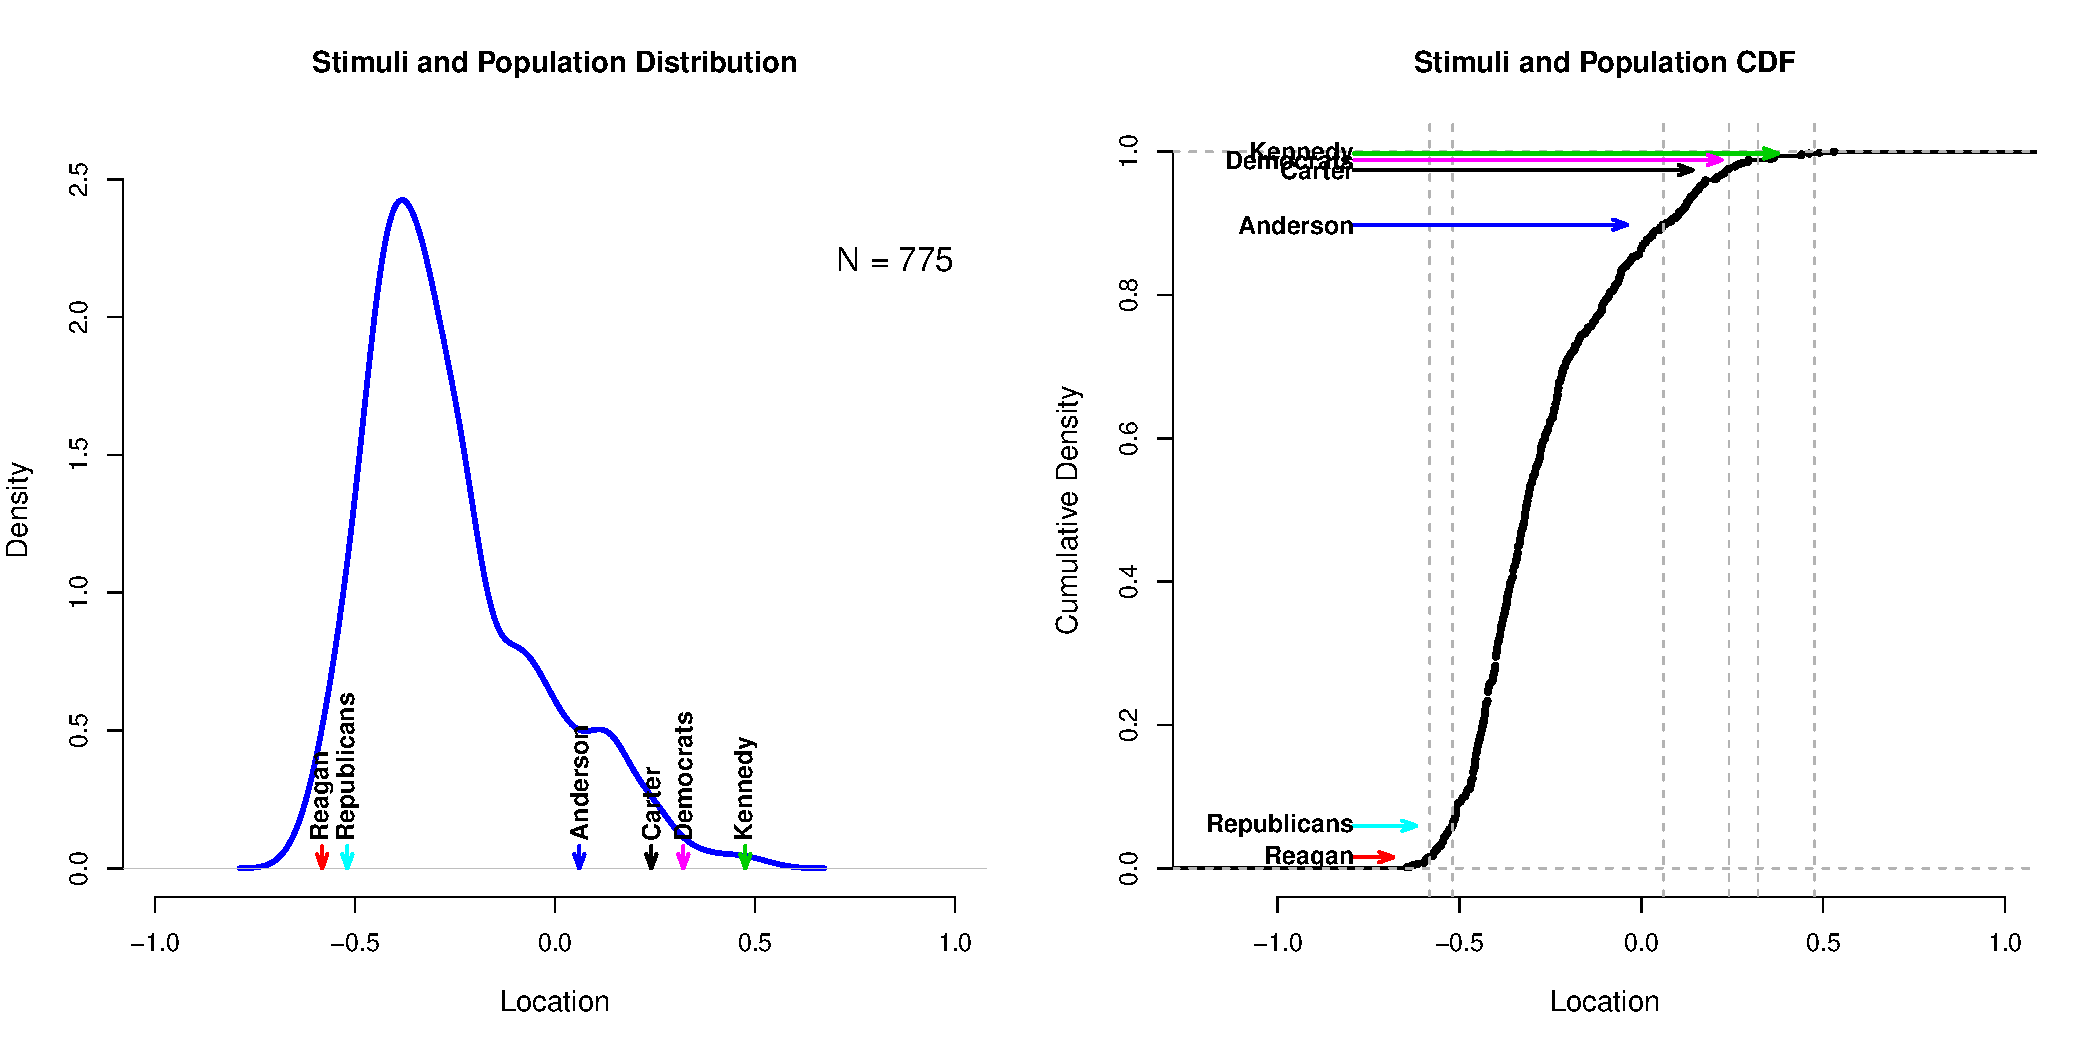
\includegraphics{basicspace-bbt}
\end{center}
\caption{Blackbox Transpose PDF and CDF plots.}
\label{fig:bbt}
\end{figure}

We can also produce summary reports of the stimuli as follows:

\begin{Schunk}
\begin{Sinput}
> summary(result)
\end{Sinput}
\begin{Soutput}
SUMMARY OF BLACKBOX TRANSPOSE OBJECT
----------------------------------
              N coord1D    R2
Carter      768   0.241 0.563
Reagan      765  -0.582 0.822
Kennedy     754   0.476 0.648
Anderson    689   0.061 0.230
Republicans 771  -0.519 0.757
Democrats   774   0.321 0.651

              N coord1D coord2D    R2
Carter      768   0.238  -0.407 0.720
Reagan      765  -0.580  -0.101 0.839
Kennedy     754   0.481   0.013 0.680
Anderson    689   0.059   0.864 0.946
Republicans 771  -0.518  -0.117 0.767
Democrats   774   0.321  -0.252 0.718

              N coord1D coord2D coord3D    R2
Carter      768   0.191  -0.261  -0.663 0.918
Reagan      765   0.216   0.556   0.141 0.856
Kennedy     754   0.162  -0.510   0.697 0.981
Anderson    689  -0.911   0.053  -0.002 1.000
Republicans 771   0.210   0.498   0.055 0.780
Democrats   774   0.131  -0.335  -0.228 0.765

	Dimensions Estimated: 3
	Number of Rows: 6
	Number of Columns: 775
	Total Number of Data Entries: 4521
	Number of Missing Entries: 129
	Percent Missing Data: 2.77%
	Sum of Squares (Grand Mean): 12683.93
\end{Soutput}
\end{Schunk}


\section{Example 3: Aldrich and McKelvey's Estimator}

The transposed basic space model is a generalization of a model developed by \citet{aldrich1977method}, which was restricted to analyzing matrices with no missing values in only one dimension.  For historical purposes, we include the original Aldrich-McKelvey estimator with this package. In the basic Aldrich-McKelvey model, the estimator assumes that:

$$Y_{ij} = Z_j + \epsilon_{ij}$$

\noindent where $Z_j$ is the true location of $j$ and $\epsilon_{ij}$ is a random variable with mean 0, positive variance that is independent of $i$ and $j$ (homoskedastic), and zero covariance across the $i$'s and $j$'s. Aldrich and McKelvey then introduce two distortion parameters, $c_i$ and $w_i$, that transform the perceived candidate position into a reported candidate position $Z_{ij}$, according to:

$$Z_{ij}= \frac{1}{w_i}(Y_{ij} - c_i)$$

A least-squares minimization procedure is then used to obtain estimates of $\{Z_j\}_{j=1}^{J}$ and $\{w_i,c_i\}_{i=1}^{I}$.

We begin by reestimating the earlier results using the 1980 Liberal-Conservative scales using the Aldrich-McKelvey estimator. While the \code{aldmck} function accepts nearly identical arguments the \code{blackbox\_transpose}, one notable difference appears by default.  \code{aldmck} also accepts a column in the data matrix, specified by the \code{respondent} argument, that specifies the respondent's self placement on the issue scale. The reported respondent rating is then transformed into an ideology score by applying the respondent's personal stretch and bias parameters to that score. Note that the results largely correspond to those shown earlier with \code{blackbox\_transpose}.

\begin{Schunk}
\begin{Sinput}
> data(LC1980)
> result <- aldmck(data = LC1980, polarity = 2, 
+     respondent = 1, missing = c(0, 8, 9), verbose = TRUE)
\end{Sinput}
\begin{Soutput}
	Beginning Aldrich-McKelvey Scaling...

		Column 'Self' is set as the self placement.
		Column 'Carter' is set as the left-leaning stimulus.
		646 of 888 observations are complete.
		6 stimuli have been provided.

	Aldrich-McKelvey estimation completed successfully.
\end{Soutput}
\begin{Sinput}
> summary(result)
\end{Sinput}
\begin{Soutput}
SUMMARY OF ALDRICH-MCKELVEY OBJECT
----------------------------------

Number of Stimuli: 6
Number of Respondents Scaled: 643
Number of Respondents (Positive Weights): 569
Number of Respondents (Negative Weights): 74

R-Squared: 0.65
Reduction of normalized variance of perceptions: 0.14 

            Location
Kennedy       -0.485
Democrats     -0.317
Carter        -0.232
Anderson      -0.065
Republicans    0.517
Reagan         0.582
\end{Soutput}
\end{Schunk}



\begin{figure}
\begin{center}
\begin{Schunk}
\begin{Sinput}
> plot.aldmck(result)
\end{Sinput}
\end{Schunk}
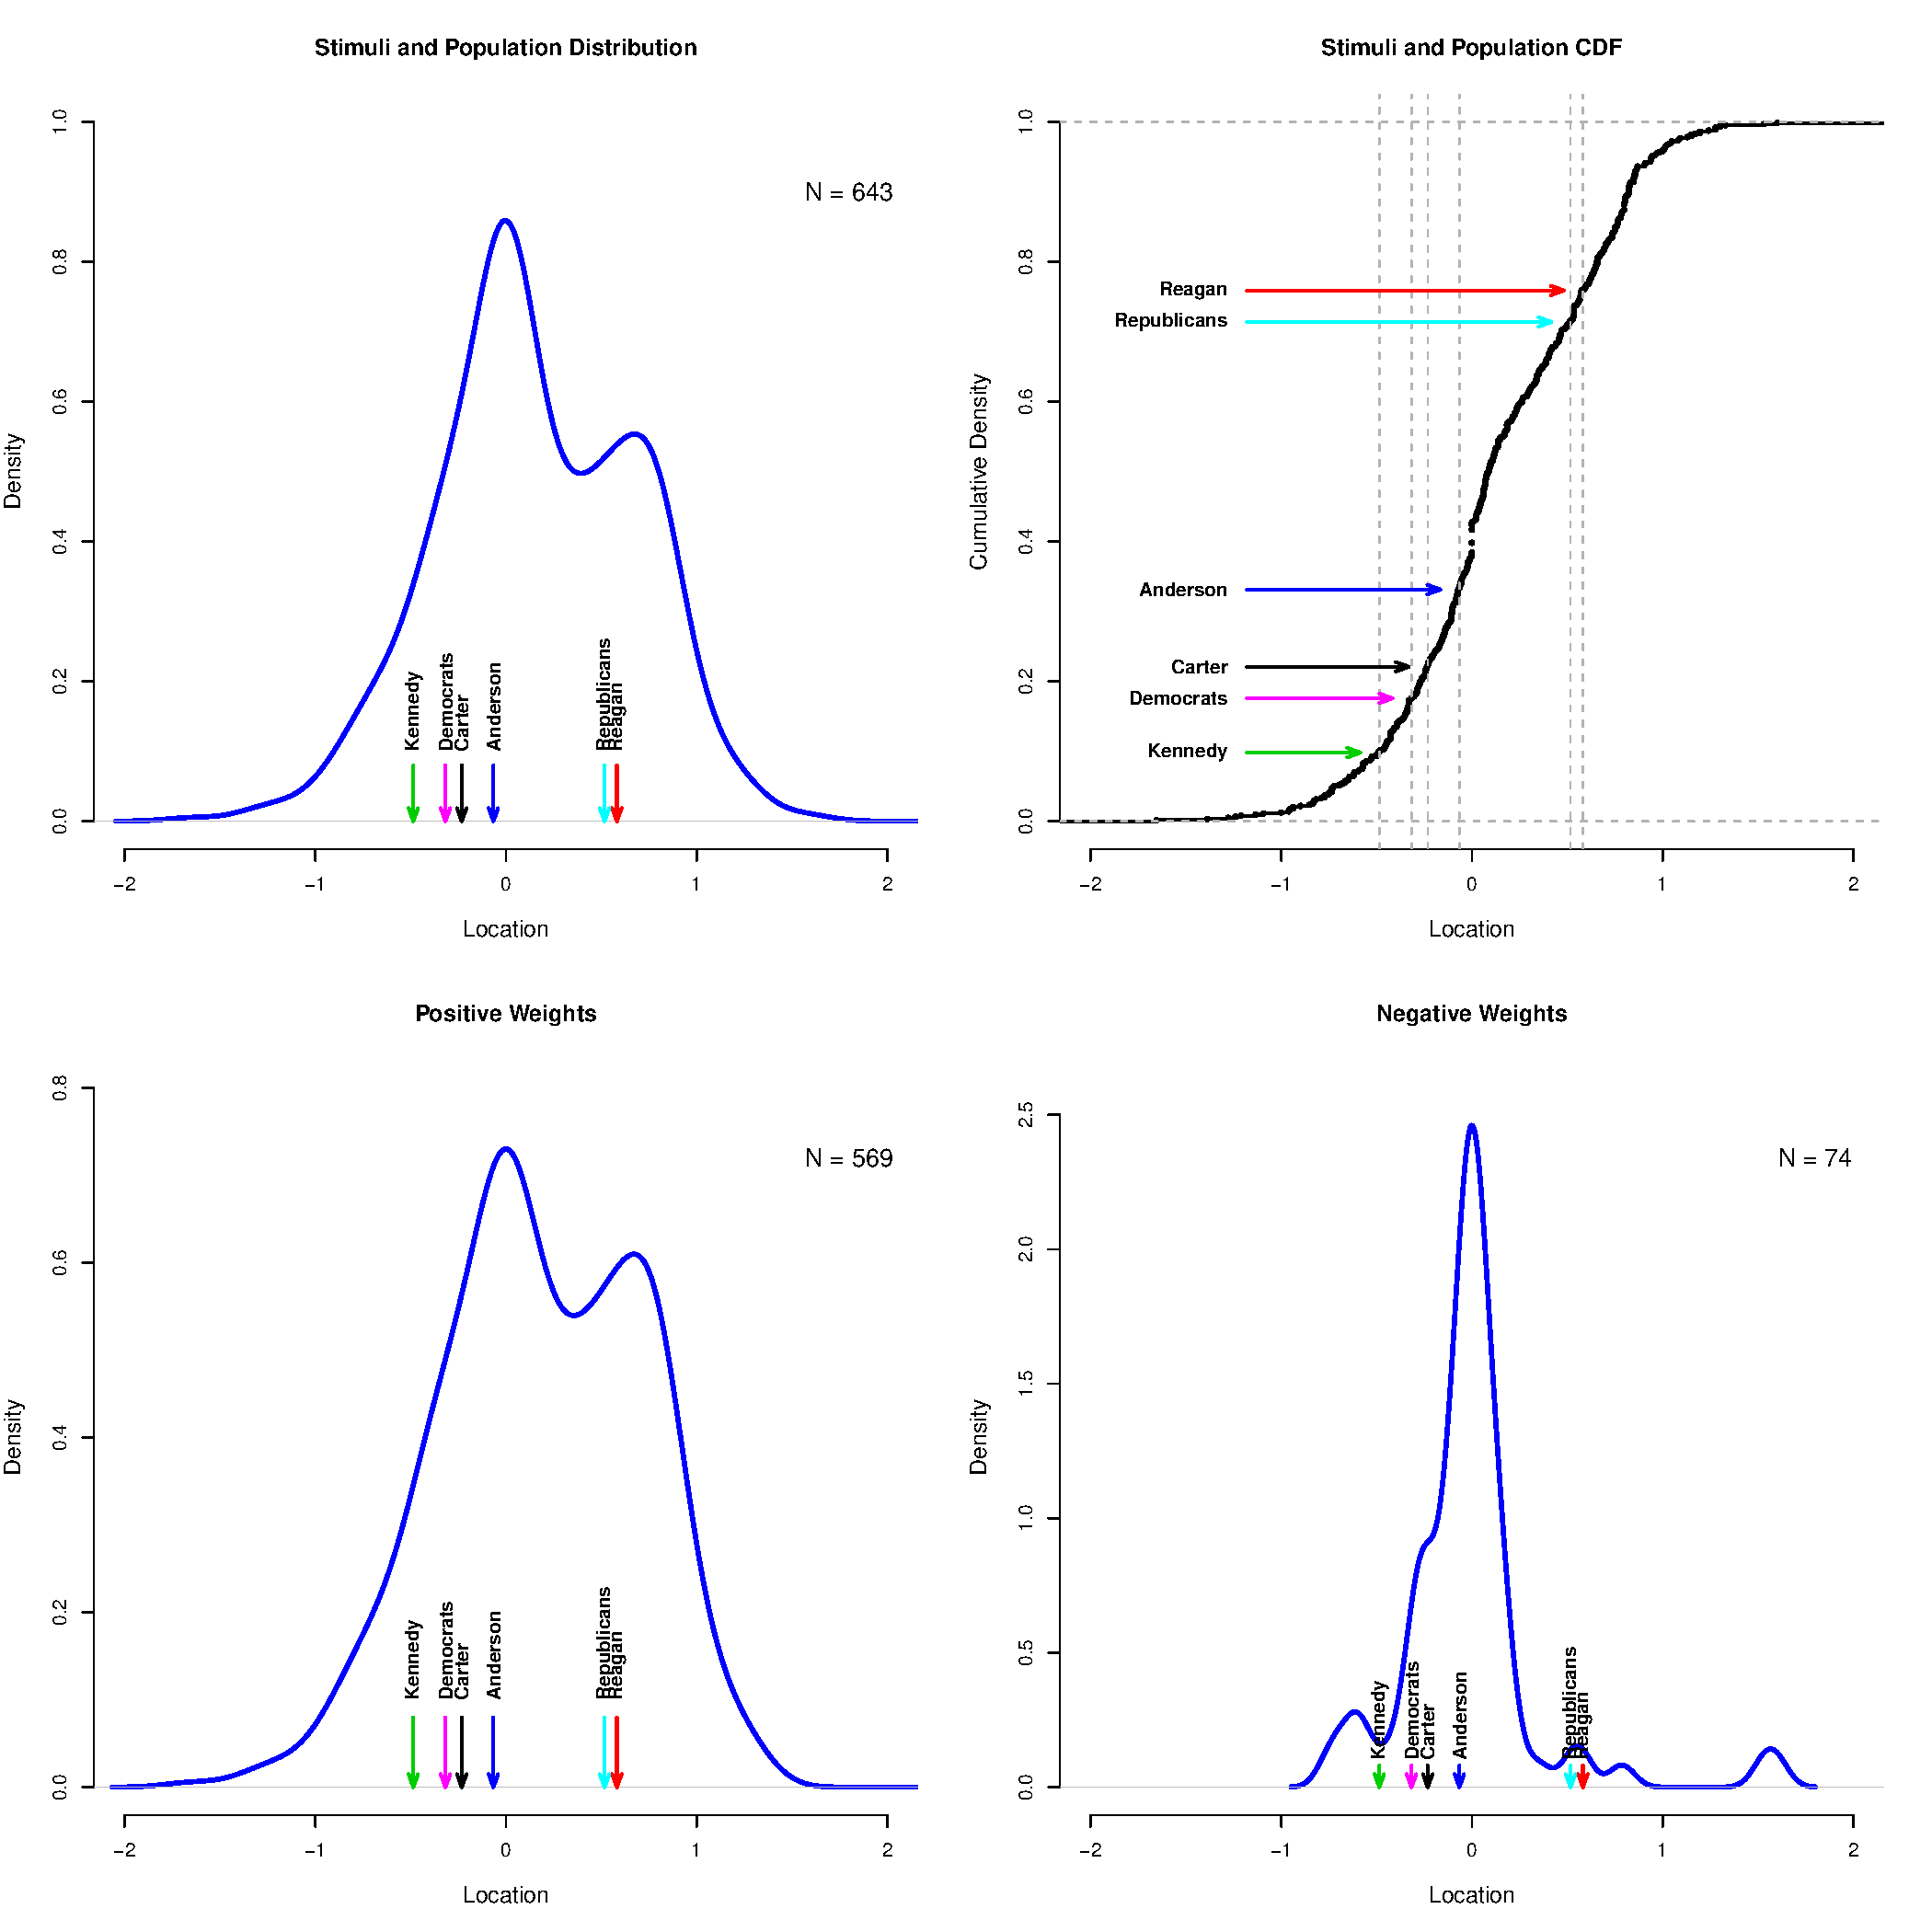
\includegraphics{basicspace-aldmck_plot}
\end{center}
\caption{Aldrich-McKelvey plots.}
\label{fig:aldmck_plot}
\end{figure}



Estimation of uncertainty for estimates using Aldrich-McKelvey can be obtained via the non-parametric bootstrap \citep{efron1993introduction}. To simulate 20 samples from the 1980 Liberal-Conservative scales, we do the following:

\begin{Schunk}
\begin{Sinput}
> Ntrials <- 20
> results <- vector("list", Ntrials)
> for (i in 1:Ntrials) results[[i]] <- aldmck(data = LC1980[sample(nrow(LC1980), 
+     nrow(LC1980), replace = TRUE), ], polarity = 2, 
+     respondent = 1, missing = c(0, 8, 9), verbose = FALSE)
\end{Sinput}
\end{Schunk}

The Aldrich-McKelvey function is primarily intended for scaling perceptual data from surveys, though it can also be used to replicate previously published Monte Carlo results from \citet{palfrey1987relationship}. Palfrey and Poole find that the Aldrich-McKelvey algorithm is robust to the assumption of homoskedastic error, and test this by replacing the homoskedastic error term $\epsilon_{ij}$ with a respondent-specific $\epsilon_{i}$. In this example we replicate their result in a single trial, and show that the estimated rank ordering of the stimuli $\hat{Z_j}$ is identical to the true $Z_j$.

\begin{Schunk}
\begin{Sinput}
> Nstimuli <- 6
> Nresp <- 500
> Z_j <- rnorm(6)
> Z_j <- (Z_j - mean(Z_j))/sd(Z_j)
> respondent.sd <- runif(Nresp, min = 0.3, max = 0.9)
> error_heteroskedastic <- matrix(NA, Nresp, Nstimuli)
> for (i in 1:Nresp) error_heteroskedastic <- rnorm(Nstimuli, 
+     sd = respondent.sd)
> w_i <- runif(Nresp, min = 0, max = 1)
> c_i <- rnorm(Nresp)
> Y_ij <- rep(1, 500) %o% Z_j
> Y_ij <- Y_ij + error_heteroskedastic
> Z_ij <- 1/w_i %o% rep(1, Nstimuli) * (Y_ij - c_i %o% 
+     rep(1, Nstimuli))
> result <- aldmck(Z_ij, polarity = 6, missing = c(999))
> rank(Z_j)
\end{Sinput}
\begin{Soutput}
[1] 2 6 5 3 4 1
\end{Soutput}
\begin{Sinput}
> rank(result$stimuli)
\end{Sinput}
\begin{Soutput}
2 6 5 3 4 1 
\end{Soutput}
\end{Schunk}

Although we only show one trial in this paper, the result shown here is robust to tests over multiple simulations.\footnote{Replication of the Monte Carlo test with separate groups of informed and uniformed individuals, from \citet[pg. 515]{palfrey1987relationship}, can be conducted by simply changing the respondent's error deviations in the code above to have 250 respondents with $\sigma_i=0.3$ and 250 respondents with $\sigma_i=0.9$.}

\section{Conclusion}

Social scientists often wish to infer the locations of voters and legislators in an abstract policy or ideological space.  In situations where this cannot be accomplished with a preference data-oriented estimator such as NOMINATE \citep{Congress}, the use of perceptual data-oriented estimators such as the basic space technique described here are a useful alternative. Given the abundance of perceptual data questions found in most social science surveys, we believe there are many possible applications of this estimator. By providing an R \citep{R} package that facilitates the analysis of perceptual data in a popular statistics environment, we hope to encourage a renewed interest in this important literature.

\section{Acknowledgments}

This research was supported by a grant from the National Science Foundation (NSF-SBS-0611974). James Lo also acknowledges support from SFB 884, ``Political Economy of Reforms''.

\newpage

\bibliography{basicspace}

\end{document}

